\chapter{State of art}
In this chapter is presented the current implementation to support edge and fog computing paradigms within the energy production and monitoring network, based on the Smart Grid model (translating hardware components into an IT network) and the use of the Kubernetes platform. The limitations that the implementation studied in this thesis aims to eliminate will also be highlighted.

\section{Smart Grid components}
Currently, the Smart Grid model of the energy monitoring network consists of the Area Control Center, which is the central hub for control and decision-making mechanisms, and the production and distribution stations, which are divided into primary and secondary. To manage the network, three main applications are used: Phasor Measurement Units (PMU) for measurements, Phasor Data Concentrator (PDC) from the openPDC project for aggregating data from various PMUs, and Grid State Estimation (GSE) for monitoring the network based on the data provided by the previous applications. A graphical example of the Smart Grid model is shown in the figure \ref{fig:art-state}.
\begin{figure}[ht]\centering
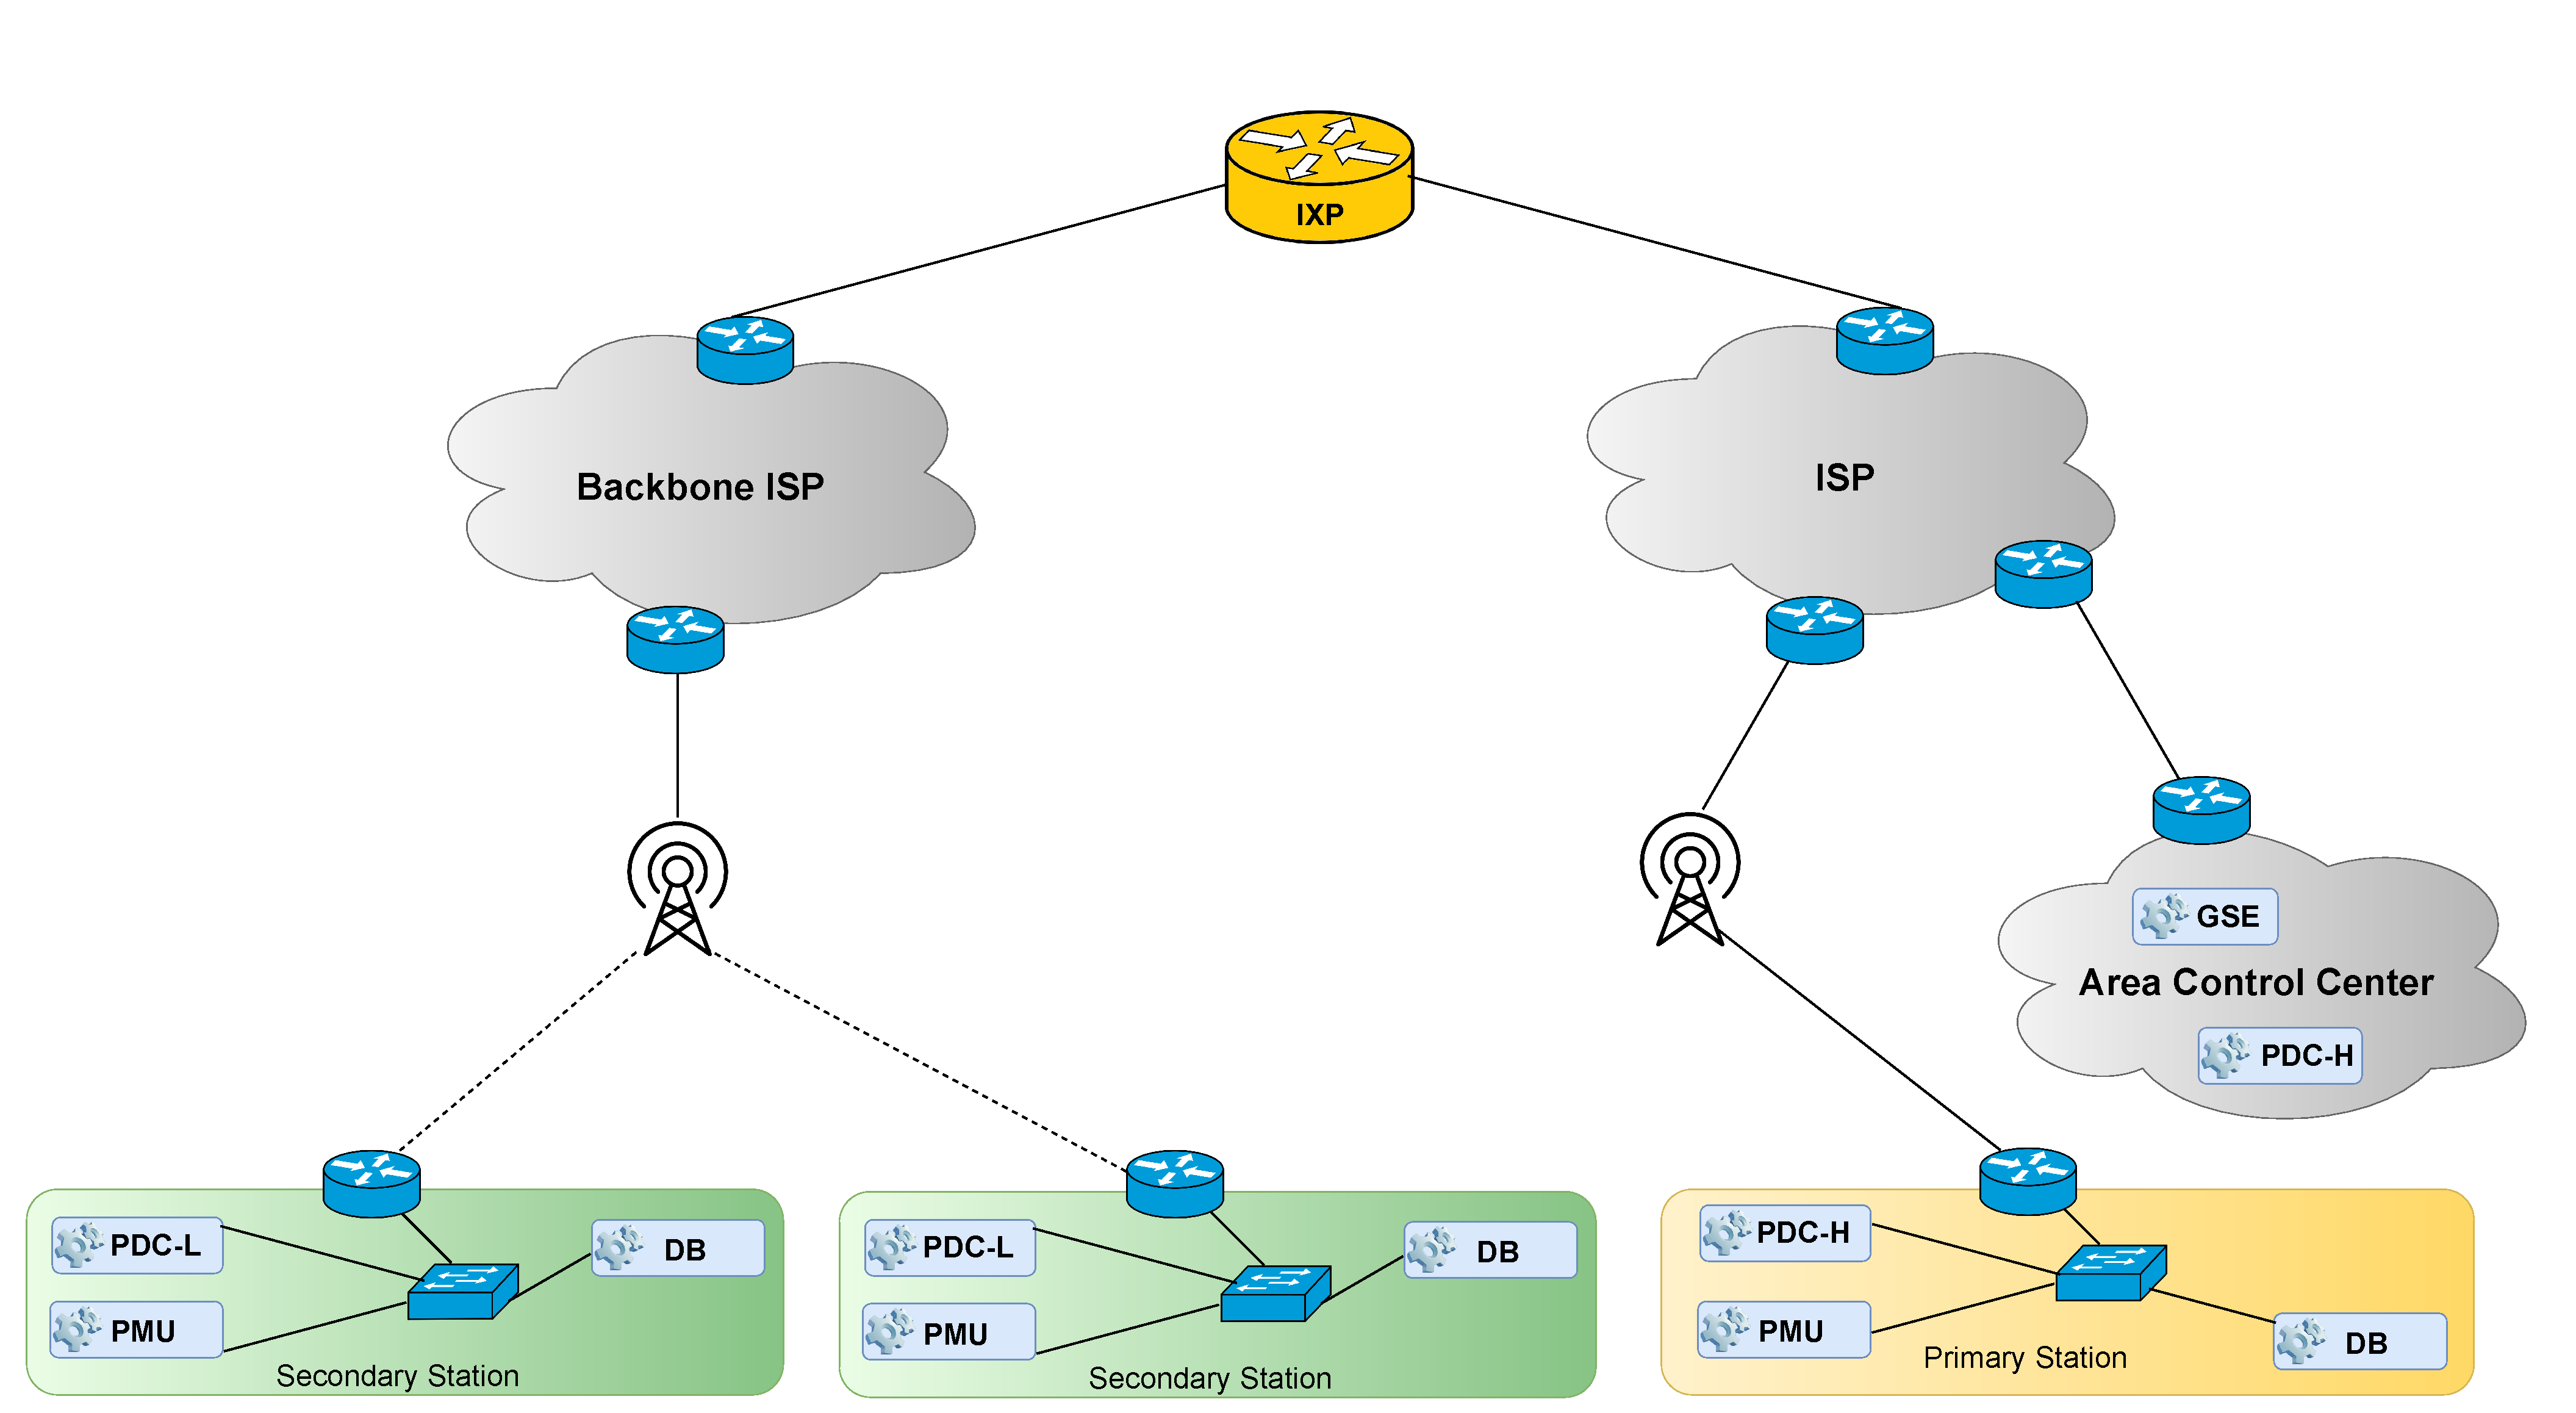
\includegraphics[scale=0.17]{Pictures/state-of-art}
\caption{Smart Grid abstract informatic model}\label{fig:art-state}
\end{figure}

\subsection{Area Control Center}
A computing node, in the optic of Smart Grid, that represents an Operational Distribution Center, thus housing the control and management logic of the entire network. This node typically manages the high-level PDC, where data streams from other high-level PDCs located at primary stations are aggregated, and the GSE application, which uses the data from the previous PDC to control the network.

\subsection{Station}
A computing node, in the optic of Smart Grid, that represents an energy production or distribution station. Primary stations primarily use a high-level PDC to aggregate data streams from their subnet of secondary stations but can also manage some PMUs. Secondary stations mainly handle the PMUs or aggregate the data streams produced by those through low-level PDCs.

\subsection{Phasor Measurement Units}
PMUs provide measurements of fundamental electrical quantities, such as voltage and current, in the form of phasors, including information on the amplitude and phase of the measured quantities. These measurements, synchronized via GPS and sampled at a frequency of 50 samples per second, enable precise monitoring of rapid changes in the electrical system caused by the dynamism of distributed energy resources.

PMUs offer a detailed perspective of system dynamics, overcoming the limitations of more traditional Remote Terminal Units (RTUs), which have an update period of several seconds and are not synchronized. The use of PMUs is expected to enhance the observability and reliability of the distribution system.

\subsection{Phasor Data Concentrator}
A phasor data concentrator (PDC) is designed to receive streaming synchrophasor data from phasor measurement units (PMUs) installed on power transmission lines and align these data using GPS timestamps (i.e., it "concentrates" the data based on time). The output of a PDC is a time-synchronized data set that is forwarded to one or more software applications.

openPDC is a flexible platform for high-speed time-series data processing, both in real-time and historically. It does not have significant computational power requirements, so it can be installed anywhere within the synchrophasor infrastructure, including on fanless computers located in substations.

\subsection{Grid State Estimation}
State estimation is a technique that allows for the reconstruction of network states, such as nodal voltages, based on available measurements and the electrical network model. Unlike traditional meters, PMU measurements, which include the phase relative to an absolute reference, simplify the state estimation problem by making it a linear system and significantly reducing the computational load. The objectives of state estimation include the recognition and reduction of measurement errors, the identification of topology errors, the estimation of unmeasured network quantities, and the determination of network parameters through redundant measurements.

\section{Multi-master station architecture}
The current state of research has advanced to managing a single node/place of the Smart Grid through a multi-master architecture \cite{a2-1}\cite{a2-2}, leveraging the resilience gained from the ability to withstand the failure of a master node, albeit at the cost of increased resources required for replicated control-plane components.

In the cluster, the configuration of applications (for example, the configuration of a PDC if the cluster represents a station) is stored in a high-availability distributed database system. This enables the quick and automatic redeployment to another node in the cluster in case of a failure, without the need to reconfigure the parameters for that application. In this way, the clusters support the automatic local resolution of failures for both applications and the nodes on which they are deployed.

Depending on the location, each cluster represents a point of edge (if managing a secondary station) or fog (if managing a primary station) computing within the Smart Grid, but the overall control architecture is manually established between each pair of clusters, which exist as completely independent separate entities.

\section{Actual challenge}
While this approach of a multi-cluster kubernetes is effective for managing a single station, it proves suboptimal when applied to an entire electrical control system. This is due to both the complexity involved in managing a large number of nodes (with stations alone numbering in the tens of thousands, whereas Kubernetes officially supports up to 5000 nodes \cite{a3-1}) and the fundamental inability to function in isolation. In fact, if a segment of the network underlying a master node becomes isolated from the rest of the architecture, it becomes unmanageable as the master node loses the necessary consensus to initiate new workloads (new pods to manage the isolated entities) and can only partially manage existing workloads (because it can't reschedule workloads if it fails).
The only additional failure scenario that the translated architecture can address is when an entire secondary station becomes isolated from the network, allowing the possible PDC pod affected to be relocated to another station. However, this advantage does not outweigh the drawbacks in terms of complexity,lack of scalability, and resource demands inherent in the overall architecture. These challenges can be effectively addressed by adopting Liqo technology.